\documentclass[final]{beamer}
\mode<presentation>
{
  \usetheme{Szeged}
\usecolortheme{crane}
}


\usepackage{times}
\usepackage{multicol}
\usepackage{amsmath,amssymb,amsthm}

\newtheorem{alg}{Algorithm}

\newcommand{\argmax}{\text{argmax}}
\usepackage{float, caption, subcaption}
\usepackage[english]{babel}
\usepackage[latin1]{inputenc}
\usepackage{beamerposter}  % e.g. custom size poster
  \title[Hangman]{{\veryHuge An Optimization Layer for Distributed Matrix Computations }}
  \author[Schramm \& Weitz]{{\Large Jonah Brown Cohen, Tselil Schramm, and Ben Weitz}}
\date{}

  \begin{document}
{\large
  \begin{frame}{} 

\maketitle

\vspace{-3cm}
\begin{center}
\begin{columns}[t]
\begin{column}{0.32\textwidth}

%----------------------------------------------------------------------------------

    \begin{block}{\huge Motivation}
\vspace{.5cm}

\begin{itemize}
\item Big data companies like Facebook, Netlix, or Google perform large-scale distributed matrix computations
\begin{itemize} {\large
\item Computations experience {\bf trade-offs} in accuracy vs. time or money. 
\begin{center}
\begin{figure}
\fbox{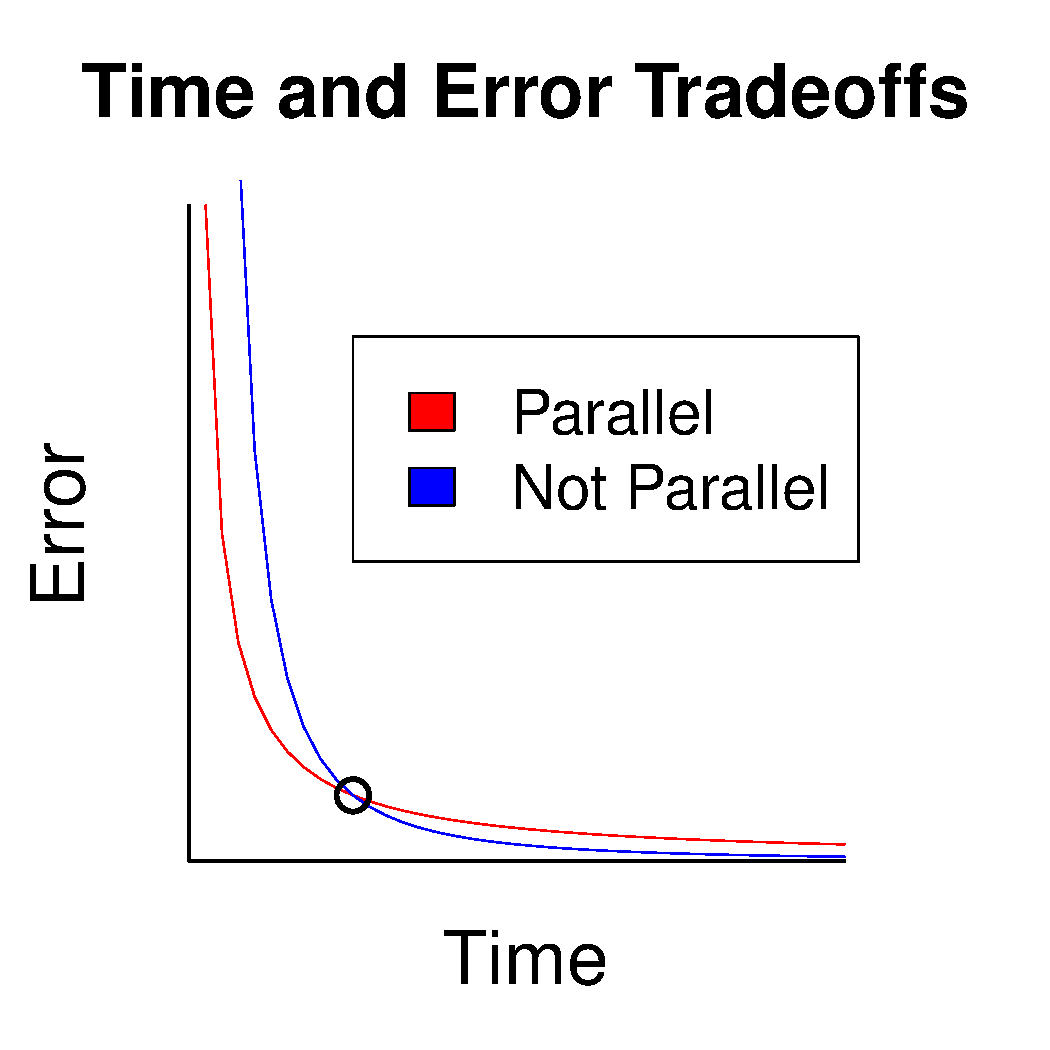
\includegraphics[width=0.35\textwidth]
{Motivations.pdf}}
\caption{Time and Error Tradeoffs}
\end{figure}
\end{center}
\item Human operators manually tweak parameters and partitioning
\item Humans are prone to error and costly to hire!
}
\end{itemize}
\item Solution: Build an optimization layer to automatically tweak and manage these computations
\begin{itemize} {\large 
\item Learn to adjust parameters from past computations
\item Incoming jobs come with budgets of time or accuracy that must be met
}
\end{itemize}
\end{itemize}

\end{block}
\vspace{1.2cm}

    \begin{block}{\huge Objective}
\vspace{.4cm}
\begin{itemize}
\item {\bf \large Create an optimizer that automatically picks algorithm parameters and the degree of data partitioning to meet budget specifications}
\end{itemize}

\vspace{.5cm}

\end{block}

\vspace{1.2cm}

    \begin{block}{\huge Framework}
\vspace{.1cm}
\begin{columns}[t]
\begin{column}{0.4\textwidth}
\begin{itemize}
\item Optimizer interface to user: input data, methods to run, and time, error, and financial budgets
\item Optimizer then interfaces with matrix algorithms implemented within a parallel framework (such as an algorithm wirtten in SparkR or methods from MLBase)
\item All parameter selection hidden from user
\end{itemize}    
\end{column}
\begin{column}{.6\textwidth}
\begin{center}
\begin{figure}
\fbox{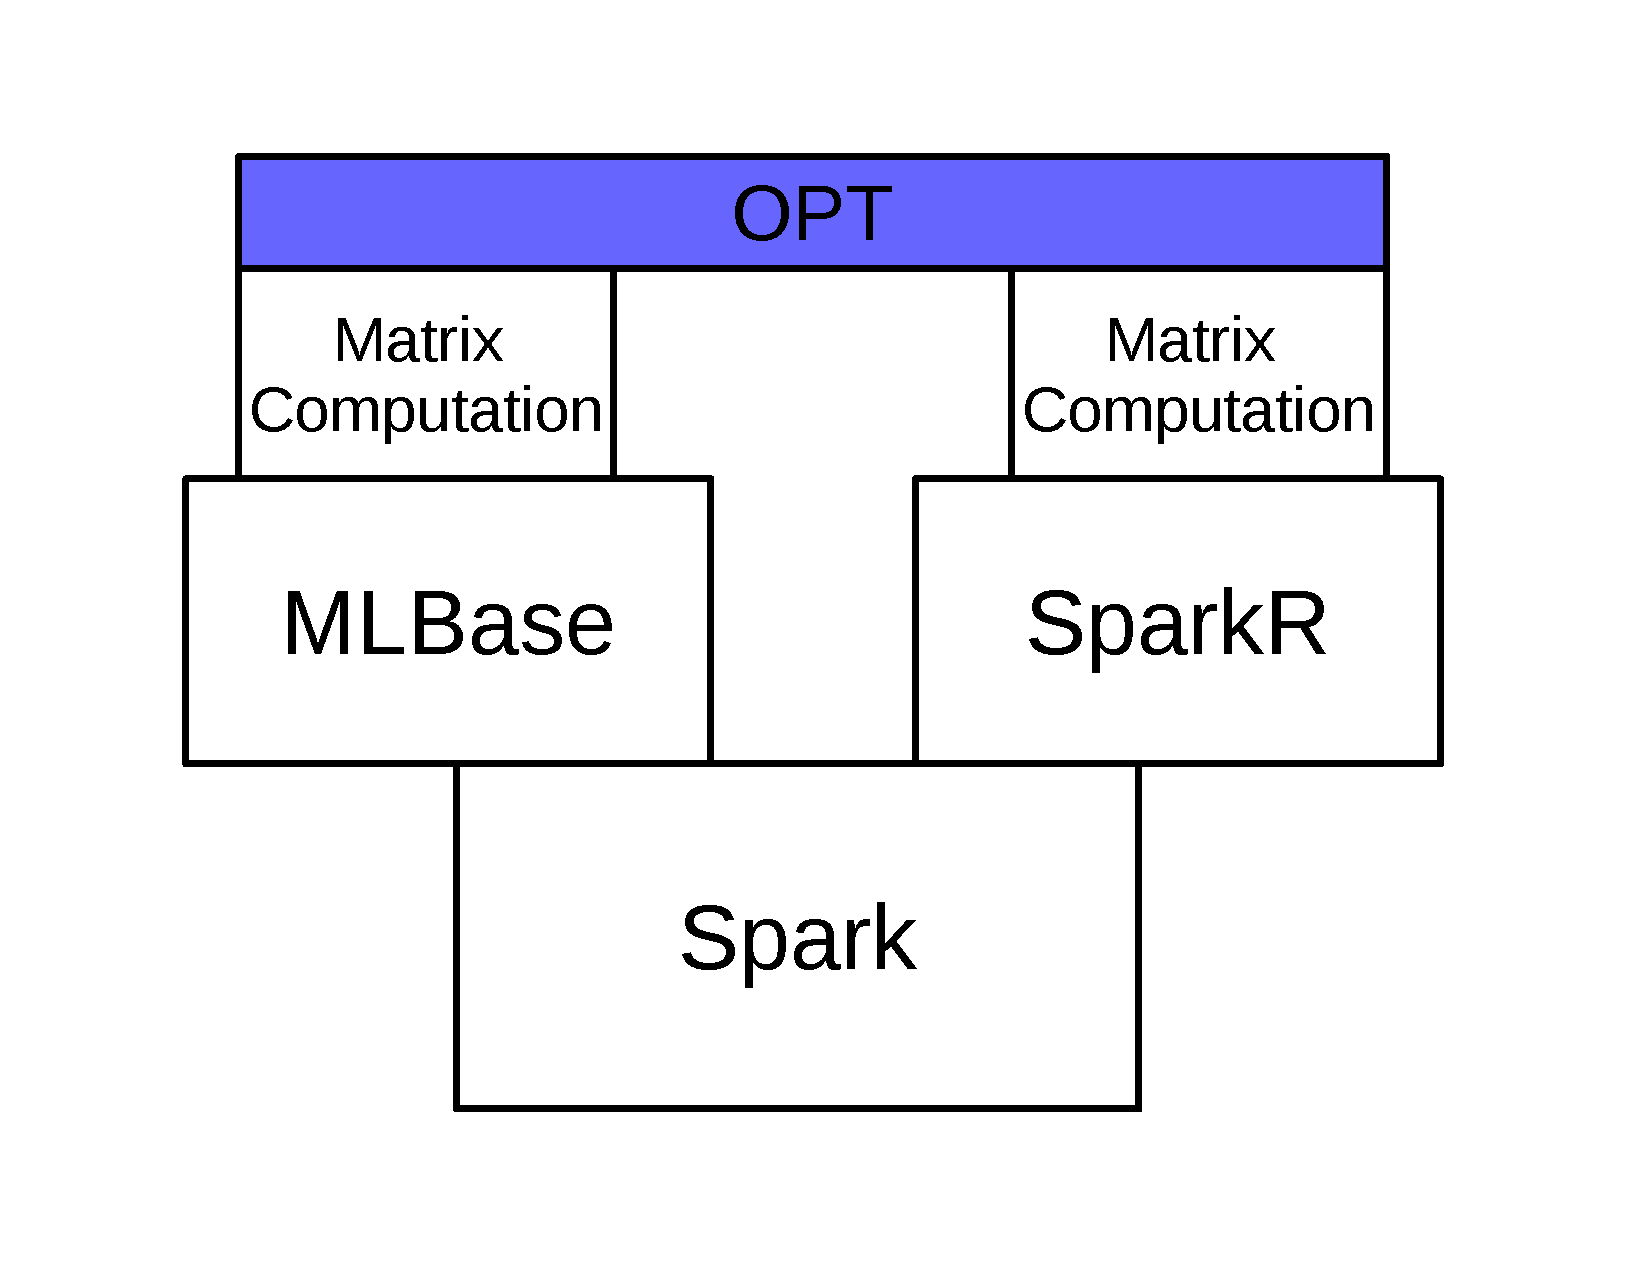
\includegraphics[width=0.75\textwidth]
{SysDiagram.pdf}}
\caption[width=\textwidth]{Our optimizer provides an interface to the user, through which the user specifies the algorithm and a time, error, and monetary budget. The optimizer then calls down to the matrix computation framework with the appropriate parameters.}
\end{figure}
\end{center}
\end{column}
\end{columns}
\end{block}

%----------------------------------------------------------------------------------

\vspace{1.2cm}

   
\end{column}

\begin{column}{0.32\textwidth}
 
    \begin{block}{\huge Optimizer Design}
\vspace{.5cm}


Our optimizer is:
\begin{itemize}
\item Architecture-independent
\begin{itemize} {\large
\item Stores statistics from prior jobs on the architecture in question
\item Parameters chosen based on statistics for the specific architecture
}
\end{itemize}
\vspace{.5cm}

\item Adaptive
\begin{itemize} {\large
\item Stores statistics from previous jobs on instances with similar distribution
\item Prediction of the optimal parameters improves as the optimizer learns
}
\end{itemize}
\vspace{.5cm}

\item Avoids Local Optima
\begin{itemize} {\large
\item When one choice of parameters already encountered is slightly better, there is a risk of getting stuck at a local optimum
\item In ``explore mode'' we choose the instance parameters randomly, with probability proportional to the relative suitability of the parameters
}
\end{itemize}
\end{itemize}

\vspace{.7cm}

\begin{center}
\begin{figure}
\fbox{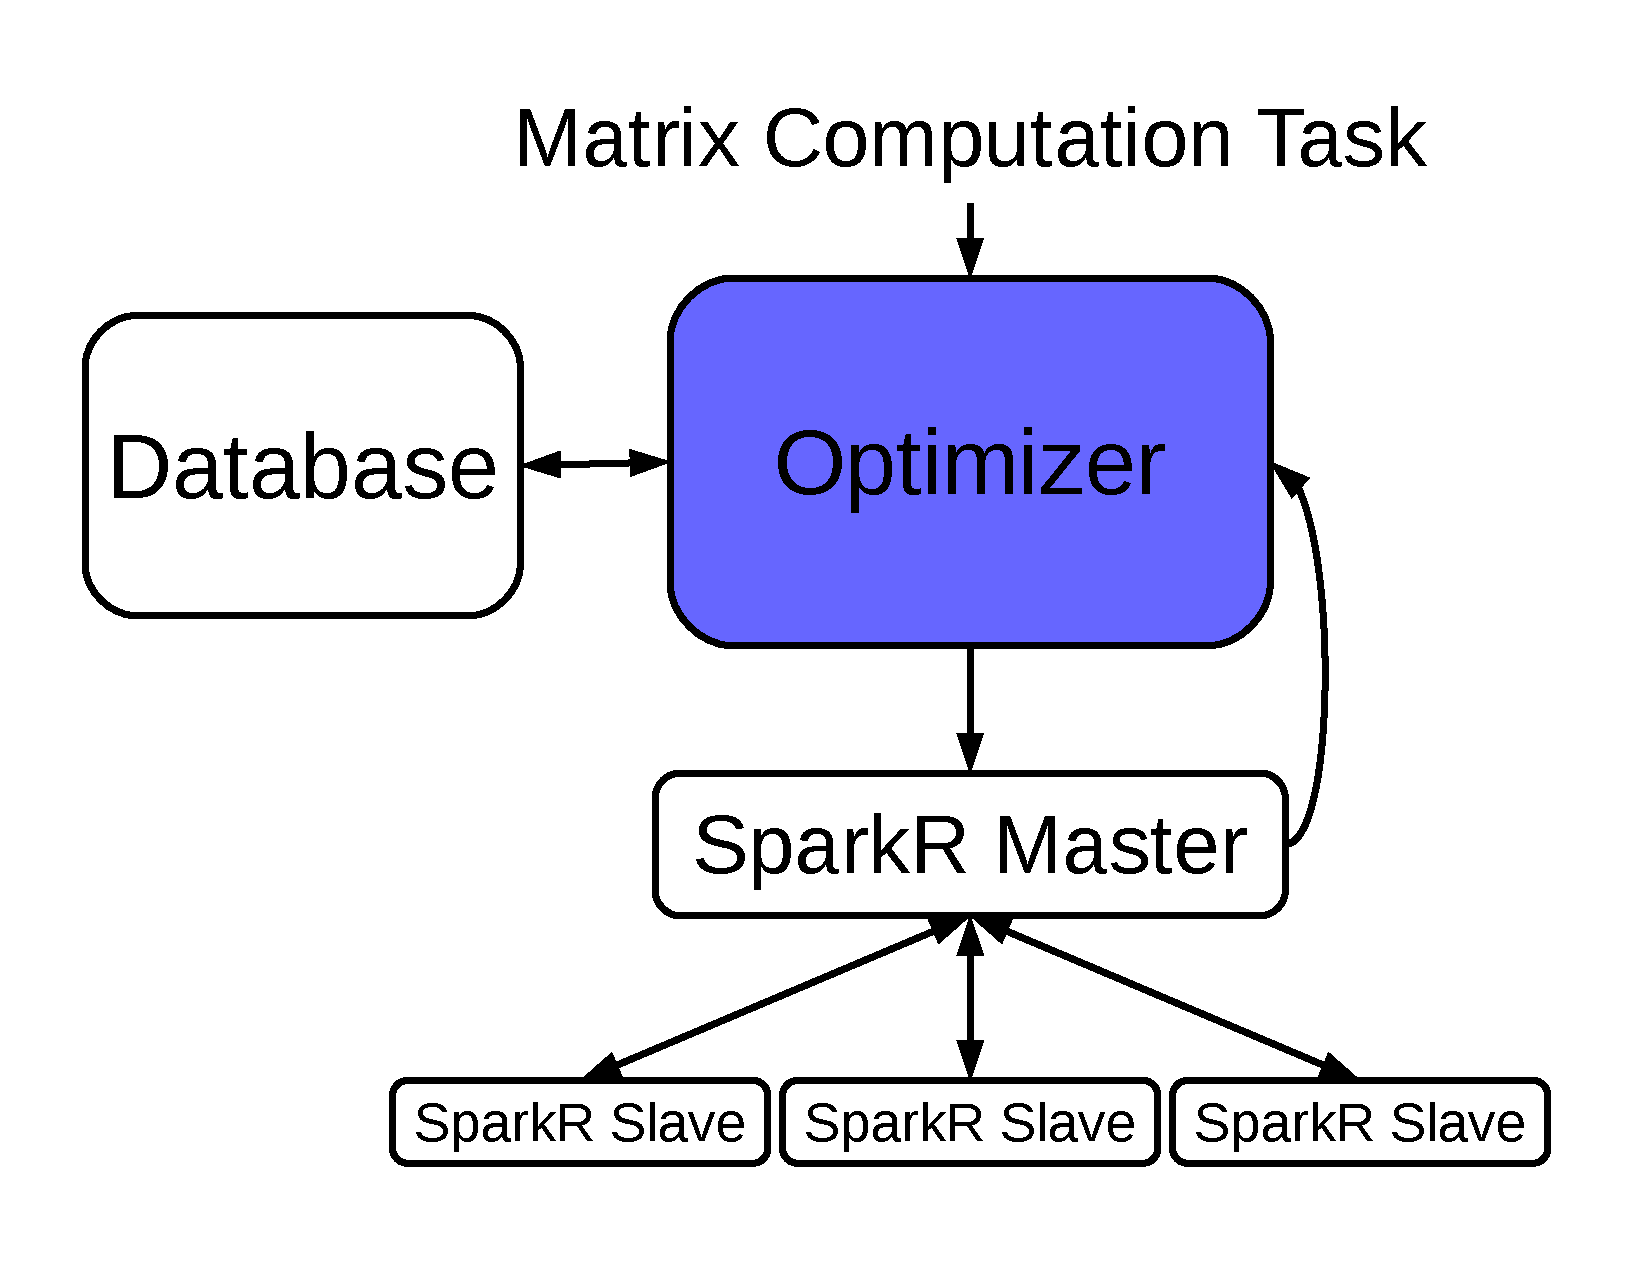
\includegraphics[width=0.6\textwidth]{BoxDiagram.pdf}}
\caption[width=0.6\textwidth]{The control flow of our optimizer. The optimizer looks up relevant information in a database, then interacts with the distributed computation framework (in our current implementation, SparkR).}
\end{figure}
\end{center}




\end{block}

\vspace{1.5cm}

    \begin{block}{\huge Implementation}

\vspace{.5cm}
\begin{itemize}
\item The matrix computation: Divide-Factor-Combine (DFC)
\vspace{.2cm}
\begin{figure}
\fbox{\includegraphics[width=0.6\textwidth]{DFC.jpg}}
\caption[width=0.6\textwidth]{DFC is a distributed matrix factorization algorithm. Image taken from http://www.cs.berkeley.edu/$\sim$ameet/dfc/}
\end{figure}
\vspace{.2cm}
\item The parallel computation framework: SparkR
\begin{itemize}{\large
\item An interface for Spark in R
}
\end{itemize}
\item Implemented DFC to be incorporated into SparkR
\item Both randomized and deterministic projection methods
\item Two different base factorization methods: APG and SGD
\end{itemize}
\vspace{.5cm}

    \end{block}


\end{column}

\begin{column}{0.32\textwidth}

       \begin{block}{\huge Evaluation}

\vspace{1cm}
{\Large Tested on Synthetic and Real-world Data}
\begin{itemize}
\item Gaussian Random Matrices
\begin{itemize} {\large
\item Trained on four random matrices and tested on a fifth}
\begin{figure}
	\begin{subfigure}[b]{.45\textwidth}
\begin{center}
		\fbox{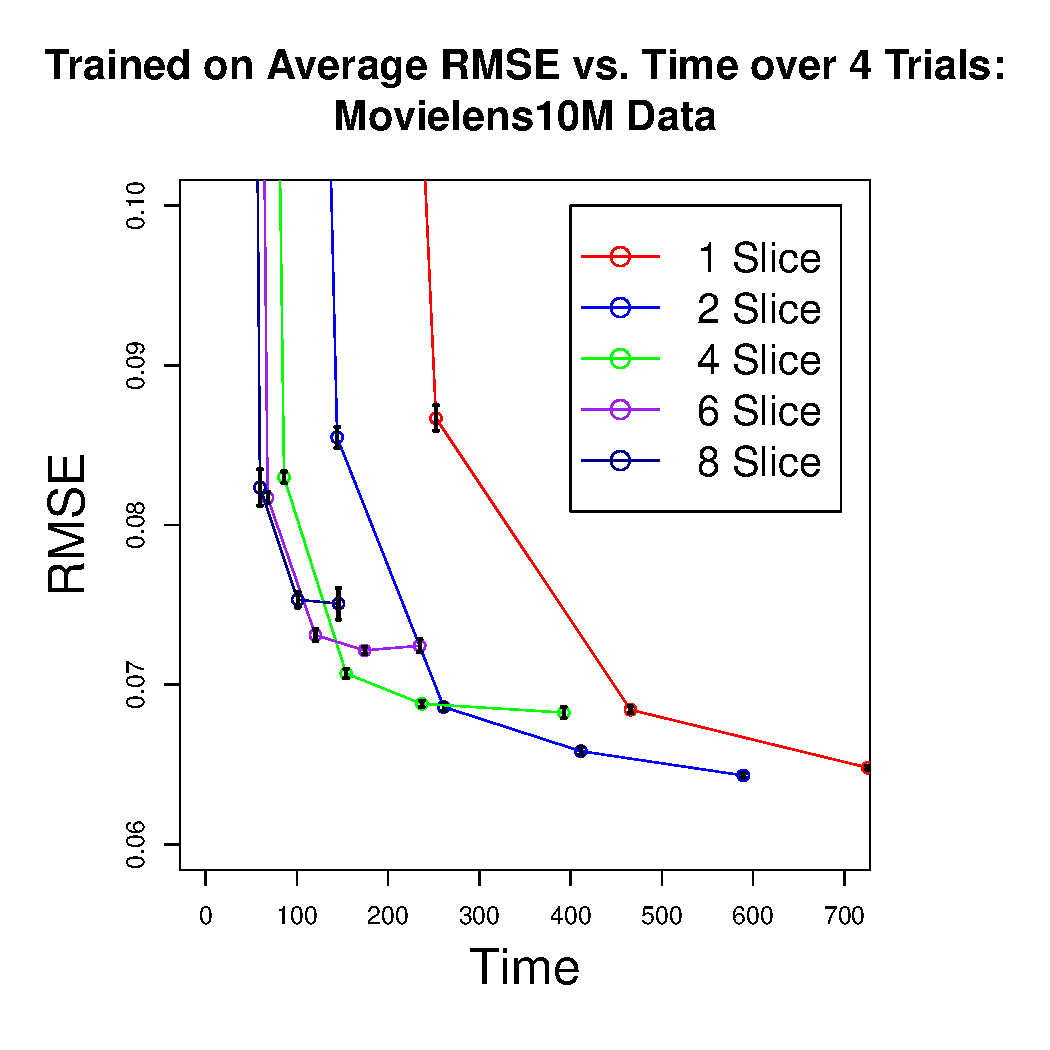
\includegraphics[width=\textwidth]{4000_90_1_to_4_RvT_graph.pdf}}
		\caption{Training Data}
\end{center}
	\end{subfigure}
\hspace{1cm}
	\begin{subfigure}[b]{.45\textwidth}
\begin{center}
		\fbox{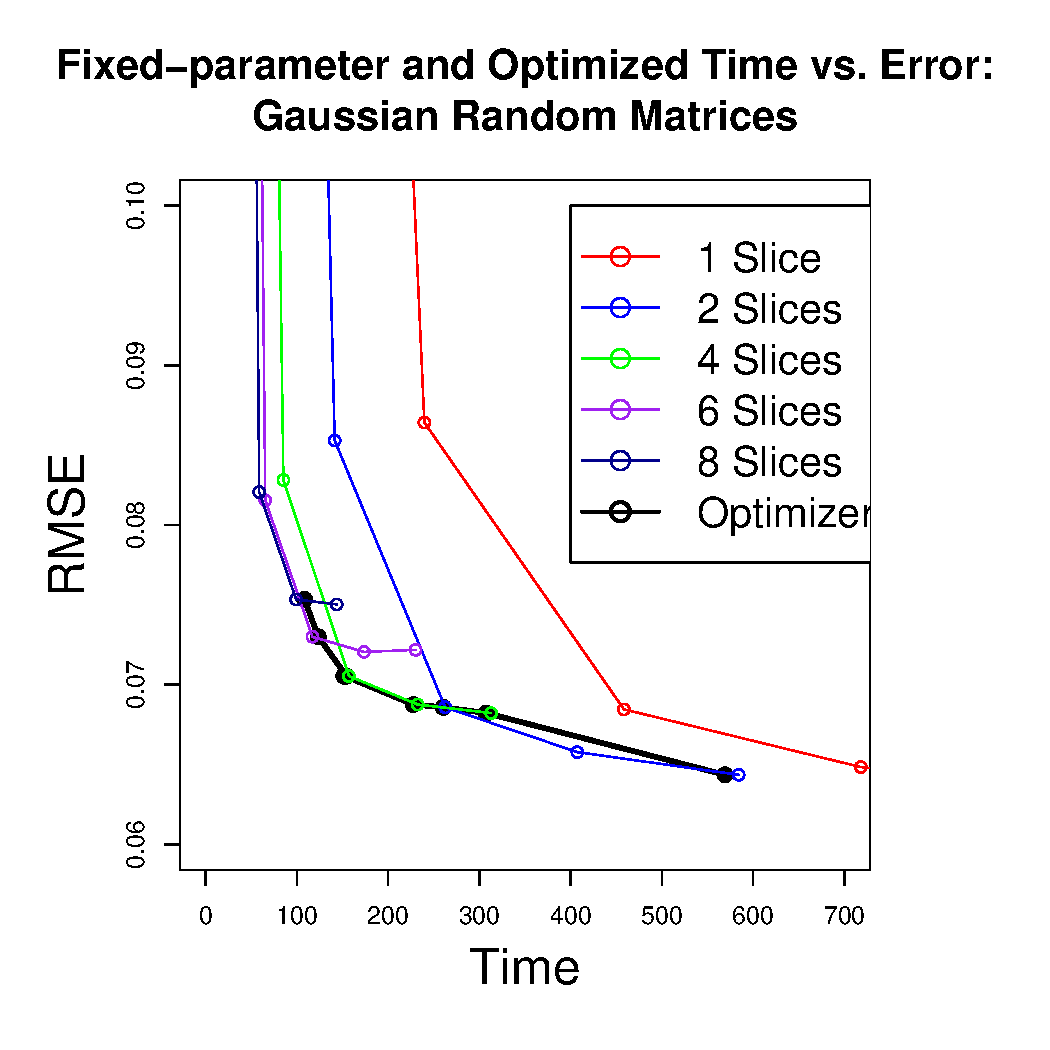
\includegraphics[width=\textwidth]{Opt_Gaussian_4000.pdf}}
		\caption{Testing Data}
\end{center}
	\end{subfigure}
\hfill
	\caption{Plots of Time and Error taken to factor a 4000 by 4000 matrix drawn from a Gaussian distribution}	
\end{figure}
\end{itemize}

\item MovieLens 10M Dataset (http://grouplens.org/datasets/movielens/)
\begin{itemize} {\large
\item Partitioned dataset into 7 parts
\item Trained on all but one partition and tested on the remainder}
\begin{figure}
	\begin{subfigure}[b]{.45\textwidth}
\begin{center}
		\fbox{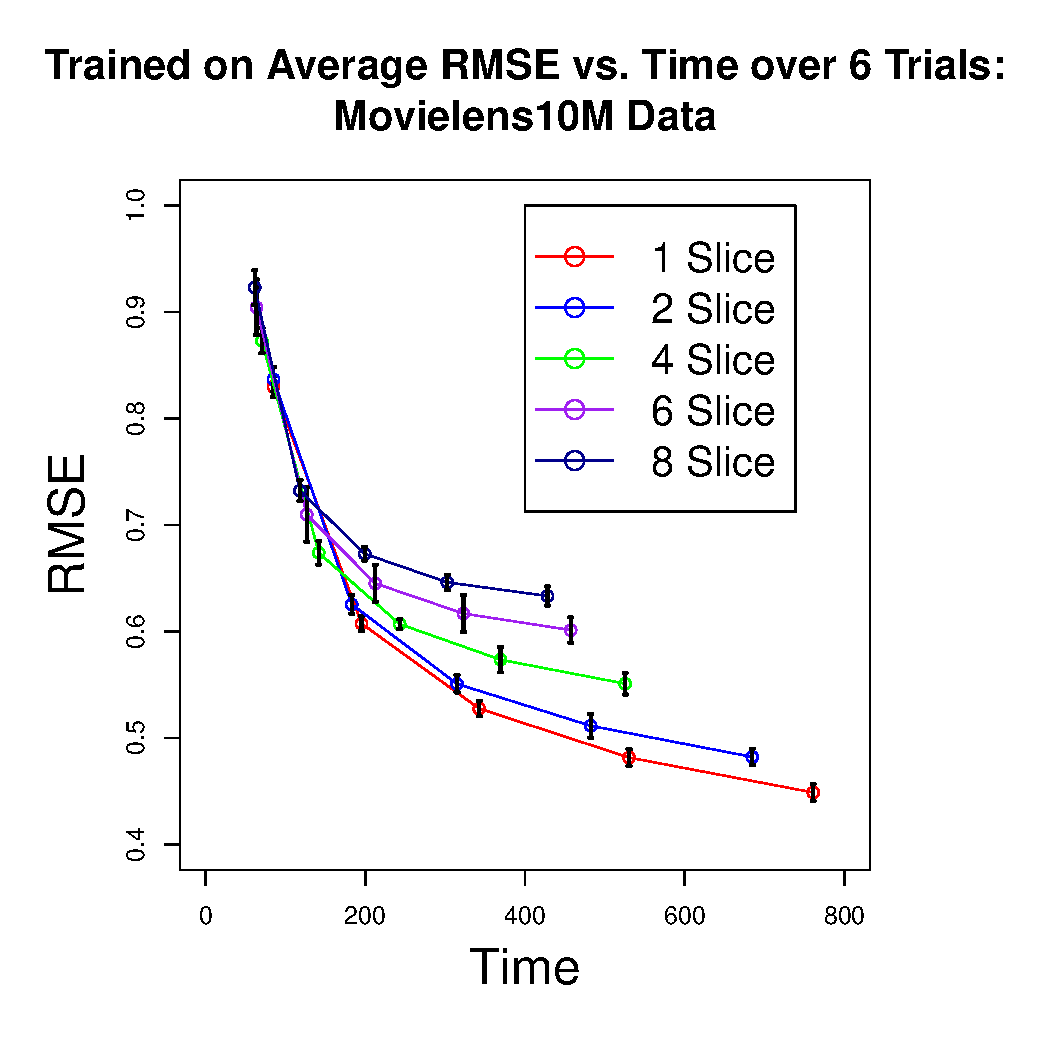
\includegraphics[width=\textwidth]{movielens10M_1_to_4_RvT_graph.pdf}}
		\caption{Training Data}
\end{center}
	\end{subfigure}
\hspace{1cm}
	\begin{subfigure}[b]{.45\textwidth}
\begin{center}
		\fbox{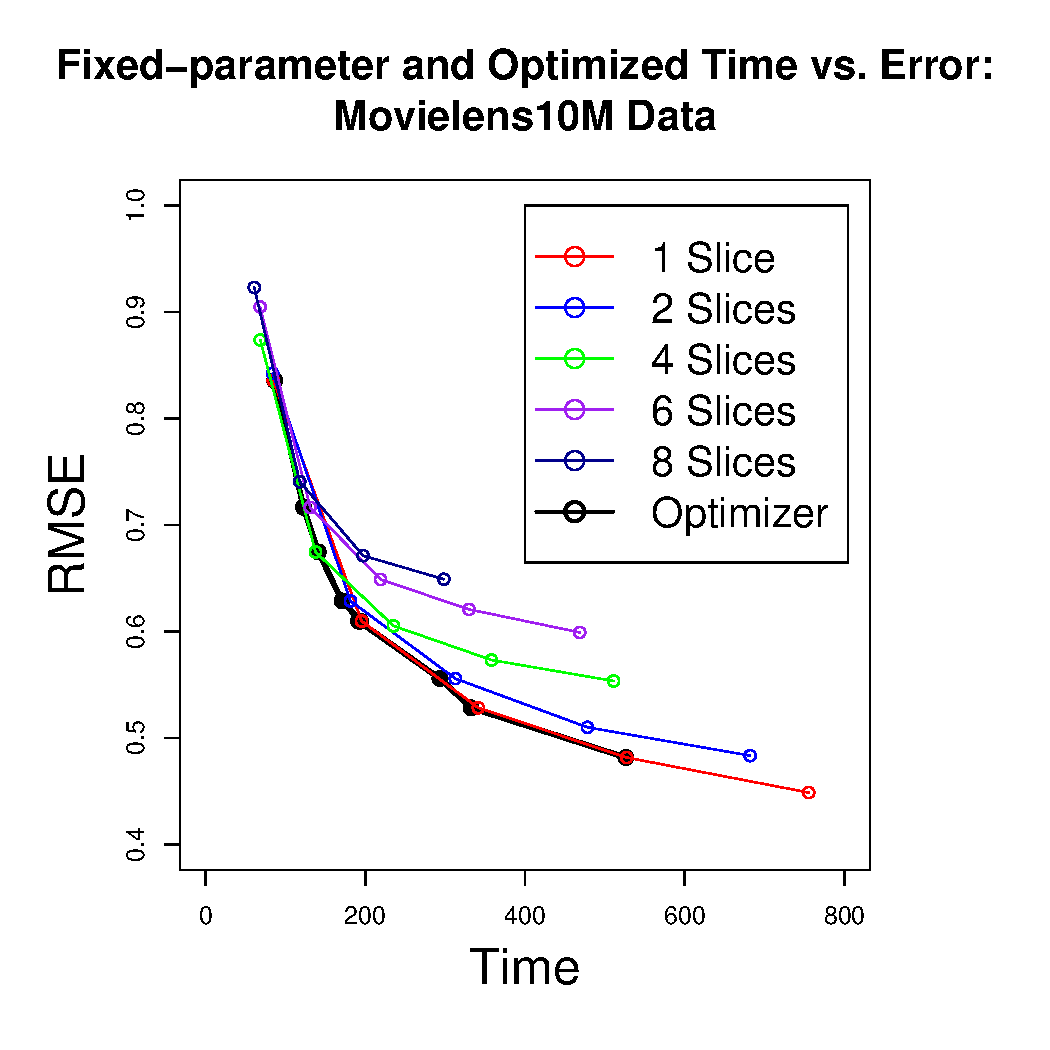
\includegraphics[width=\textwidth]{Opt_movielens.pdf}}
		\caption{Testing Data}
\end{center}
	\end{subfigure}
\hfill
	\caption{Plots of Time and Error taken to factor a partition of the Movielens10M dataset}	
\end{figure}
\end{itemize}
\item Optimizer performs as well as manually setting the parameter!
\end{itemize}

\vspace{1cm}
    \end{block}

\vspace{1.5cm}

    \begin{block}{\huge Future Work and Acknowledgements}
Some more directions for improvements include:
\begin{itemize}
\item Optimize over space of algorithms in addition to space of parameters
\item Avoid RAM bottlenecks by distributing collect step
\item Handle novel or different jobs
\end{itemize}
We would like to give very warm thanks to:
\begin{itemize}
\item Professors Anthony Joseph and John Kubiatowicz
\item Ameet Talwalkar and Shivaram Venkataraman for mentoring us
\item UC Berkeley and the NSF for providing funds and resources
\vspace{.5cm}
\end{itemize}
    \end{block}
\end{column}

\end{columns}
\end{center}
\vspace{1.5cm}
  \end{frame}
  \end{document}